%%%%%%%%%%%%%%%%%%%%%%%%%%%%%%%%%%%%%%%%%%%%%%%%%%%%%%%%%%%%%%%%%%%%%%%%%%%%%%%%%%%%%%%%%%%%%%%%%%%
%%%%%%%%%%%%%%%%%%%%%%%%%%%%%%%%%%%%%%%%%%%%%%%%%%%%%%%%%%%%%%%%%%%%%%%%%%%%%%%%%%%%%%%%%%%%%%%%%%%
%%%%%%%%%%%%%%%%%%%%%%%%%%%%%%%%%%%%%%%%%%%%%%%%%%%%%%%%%%%%%%%%%%%%%%%%%%%%%%%%%%%%%%%%%%%%%%%%%%%
\documentclass[12pt,dvipdfmx]{beamer}
%%%%%%%%%%%%%%%%%%%%%%%%%%%%%%%%%%%%%%%%%%%%%%%%%%%%%%%%%%%%%%%%%%%%%%%%%%%%%%%%%%%%%%%%%%%%%%%%%%%%%%
% pdfの栞・プロパティの字化けを防ぐ
\usepackage{atbegshi}
%\AtBeginShipoutFirst{\special{pdf:tounicode 90ms-RKSJ-UCS2}} %Windows
\AtBeginShipoutFirst{\special{pdf:tounicode EUC-UCS2}} %Linux, Mac
\usepackage{hyperref}
%%%%%%%%%%%%%%%%%%%%%%%%%%%%%%%%%%%%%%%%%%%%%%%%%%%%%%%%%%%%%%%%%%%%%%%%%%%%%%%%%%%%%%%%%%%%%%%%%%%%%%
%%%
%%% テーマの指定、省略時は default になる
%%%

 % フレームの指定、省略可
%%%%%%%%%%%%%%%%%%%%%%%%%%%% THEME
  %\usetheme{AnnArbor}
  %\usetheme{Antibes}
  %\usetheme{Bergen}
  %\usetheme{Berkeley}
  %\usetheme{Berlin}
  \usetheme{Boadilla}
  %\usetheme{boxes}
  %\usetheme{CambridgeUS}
  %\usetheme{Copenhagen}
  %\usetheme{Darmstadt}
  %\usetheme{default}
  %\usetheme{Dresden}
  %\usetheme{Frankfurt}
  %\usetheme{Goettingen}
  %\usetheme{Hannover}
  %\usetheme{Ilmenau}
  %\usetheme{JuanLesPins}
  %\usetheme{Luebeck}
  %\usetheme{Madrid}
  %\usetheme{Malmoe}
  %\usetheme{Marburg}
  %\usetheme{Montpellier}
  %\usetheme{PaloAlto}
  %\usetheme{Pittsburgh}
  %\usetheme{Rochester}
  %\usetheme{Singapore}
  %\usetheme{Szeged}
  %\usetheme{Warsaw}

% 省略可
%%%%%%%%%%%%%%%%%%%%%%%%%%%% COLOR THEME
  %\usecolortheme{albatross}
  %\usecolortheme{beetle}
  %\usecolortheme{crane}
  %\usecolortheme{default}
  %\usecolortheme{dolphin}
  %\usecolortheme{dove}
  %\usecolortheme{fly}
  %\usecolortheme{lily}
  %\usecolortheme{orchid}
  %\usecolortheme{rose}
  %\usecolortheme{seagull}
  %\usecolortheme{seahorse}
  %\usecolortheme{sidebartab}
  %\usecolortheme{structure}
  %\usecolortheme{whale}

% ヘッダ、フッタ、フレーム等を指定、省略可
  %%%%%%%%%%%%%%%%%%%%%%%%%%%% OUTER THEME
  %\useoutertheme{default}
  %\useoutertheme{infolines}
  %\useoutertheme{miniframes}
  %\useoutertheme{shadow}
  %\useoutertheme{sidebar}
  %\useoutertheme{smoothbars}
  %\useoutertheme{smoothtree}
  %\useoutertheme{split}
  %\useoutertheme{tree}

% タイトル、section, itemize/enumerate 環境、
% theorem 環境、図, 参考文献などのスタイルを指定、
% 省略可
  %%%%%%%%%%%%%%%%%%%%%%%%%%%% INNER THEME
  %\useinnertheme{circles}
  %\useinnertheme{default}
  %\useinnertheme{inmargin}
  \useinnertheme{rectangles}
  %\useinnertheme{rounded}


%\usefonttheme{}	% 省略可
%\logo{}		% 省略可

%%%%%%%%%%%%%%%%%%%%%%%%%%%%%%%%%%%%%%%%%%%%%%%%%%%%%%%%%%%%%%%%%%%%%%%%%%%%%%%%%%%%%%%%%%%%%%%%%%%
%%%%%%%%%%%%%%%%%%%%%%%%%%%%%%%%%%%%%%%%%%%%%%%%%%%%%%%%%%%%%%%%%%%%%%%%%%%%%%%%%%%%%%%%%%%%%%%%%%%
%%%%%%%%%%%%%%%%%%%%%%%%%%%%%%%%%%%%%%%%%%%%%%%%%%%%%%%%%%%%%%%%%%%%%%%%%%%%%%%%%%%%%%%%%%%%%%%%%%%
% navi. symbolsは目立たないが,dvipdfmxを使うと機能しないので非表示に
\setbeamertemplate{navigation symbols}{}

% 各種パッケージ
\usepackage{graphicx}
%\usepackage{url,cite}
\usepackage{amsmath}
\usepackage{amsthm} \theoremstyle{definition} %theorem環境が斜体になるので注意
\usepackage{amssymb} % AMS-TeX
\usepackage{setspace}

% \AtBeginSection[] % Do nothing for \section*
% { \begin{frame}<beamer> \frametitle{}
%    \tableofcontents[currentsection,subsectionstyle=hide]
%  \end{frame} } 

%appendixをページカウントしない
\newcommand{\backupbegin}{
   \newcounter{framenumberappendix}
   \setcounter{framenumberappendix}{\value{framenumber}}
}
\newcommand{\backupend}{
   \addtocounter{framenumberappendix}{-\value{framenumber}}
   \addtocounter{framenumber}{\value{framenumberappendix}} 
}

%%%%%%%%%%%%%%%%%%%%%%%%%%%%%%%%%%%%%%%%%%%%%%%%%%%%%%%%%%%%%%%%%%%%%%%%%%%%%%%%%%%%%%%%%%%%%%%%%%%%%%
% 本文・数式フォント
%\usepackage{palatino,mathpazo}
%\usepackage{times,mathptmx}
\usepackage[varg]{txfonts}
%\usepackage[varg]{pxfonts}

% \mathcal(\cal)の扱い
%\DeclareMathAlphabet{\mathcal}{OMS}{cmsy}{m}{n} %computer modern
%\DeclareMathAlphabet{\mathcal}{OMS}{txsy}{m}{n} %txfont
%\usepackage[psamsfonts]{eucal} % euler

% mathptmx時に数式モードのvをtxfontから借りる
% \DeclareSymbolFont{lettersA}{U}{txmia}{m}{it}
% \SetSymbolFont{lettersA}{bold}{U}{txmia}{bx}{it}
% \DeclareFontSubstitution{U}{txmia}{m}{it}
% \DeclareMathSymbol{v}{\mathalpha}{lettersA}{"33} %"

\usepackage{multirow}

%上線 widebar, Widebar
\usepackage{accents}
\makeatletter
\def\widebar{\accentset{{\cc@style\underline{\mskip11mu}}}}
\makeatother


%%%%%%%%%%%%%%%%%%%%%%%%%%%%%%%%%%%%%%%%%%%%%%%%%%%%%%%%%%%%%%%%%%%%%%%%%%%%%%%%%%%%%%%%%%%%%%%%%%%%%%

% 定理環境
% \newtheorem{theorem}{Theorem}
% \newtheorem{lemma}[theorem]{Lemma}
% \newtheorem{corollary}[theorem]{Corollary}
% \newtheorem{definition}[theorem]{Definition}
% \newtheorem{example}[theorem]{Example}
\newtheorem{proposition}{Proposition}
\newtheorem{remark}{Remark}

%%%%%%%%%%%%%%%%%%%%%%%%%%%%%%%%%%%%%%%%%%%%%%%%%%%%%%%%%%%%%%%%%%%%%%%%%%%%%%%%%%%%%%%%%%%%%%%%%%%%%%
% 各種コマンド定義等
\def\Fig#1{Fig.\@\ref{#1}}
\def\Table#1{Table~\ref{#1}}
\def\Eq#1{Eq.\@(\ref{#1})}
\def\Eqs#1{Eqs.\@(\ref{#1})}
\def\Thm#1{Theorem~\ref{#1}}
\def\Lma#1{Lemma~\ref{#1}}
\def\Sect#1{Section~\ref{#1}}
\def\Rmk#1{Remark~\ref{#1}}
\def\Prop#1{Proposition~\ref{#1}}
\def\Coro#1{Corollary~\ref{#1}}
\def\Def#1{Definition~\@\ref{#1}}
\def\Prob#1{Problem~\@\ref{#1}}
\def\ie{{i.\@e.\@,~}}
\def\eg{{e.\@g.\@,~}}
\def\etal{{et al.}}

% 数式環境用
\def\rank{\mathsf{rank}\, }
\def\dim{\mathsf{dim}\, }
\def\rspace{\mathsf{span}}
\def\supp{\mathsf{supp}}
%\def\vec#1{\mathbf{#1}}
\def\F{\mathbb{F}}
\def\wt{\mathsf{wt}}
\def\c{\mathcal{C}}
\def\dc{\mathcal{C}^{\perp}}
\def\d{\mathcal{D}}
\def\dd{\mathcal{D}^{\perp}}
\def\g{\mathcal{G}}
\def\dg{\mathcal{G}^{\perp}}
\def\p{\mathcal{P}}
% \def\rspace{\mathsf{span}}
\def\supp{\mathsf{supp}}
\def\ker{\mathsf{Ker\ }}

%\def\bari#1{\{\widebar{#1}\}}
\def\bari#1{\,\overline{{\!\{#1\}\!}}\,}
%\def\bari#1{\bar{\{#1\}}}
\def\vecxi{Z_{\bari{i}}}
%\def\vecsxi{\vec{z}_i}
\def\tvector{X}
\def\tpackets{X_1,\dots,X_n}
\def\mvector{S}
\def\mpackets{S_1,\dots,S_l}
\def\rvector{Y}
\def\wvector{W}
\def\cvector{C}
\def\cword{C_{1},\dots,C_{l+n}}
\def\pcword{C_{l+1},\dots,C_{l+n}}
\def\randvector{R}

\def\compmat{\Phi}

%%%%%%%%%%%%%%%%%%%%%%%%%%%%%%%%%%%%%%%%%%%%%%%%%%%%%%%%%%%%%%%%%%%%%%%%%%%%%%%%%%%%%%%%%%%%%%%%%%%
%%%%%%%%%%%%%%%%%%%%%%%%%%%%%%%%%%%%%%%%%%%%%%%%%%%%%%%%%%%%%%%%%%%%%%%%%%%%%%%%%%%%%%%%%%%%%%%%%%%
%%%%%%%%%%%%%%%%%%%%%%%%%%%%%%%%%%%%%%%%%%%%%%%%%%%%%%%%%%%%%%%%%%%%%%%%%%%%%%%%%%%%%%%%%%%%%%%%%%%
%%%
%%%  日本語フォントをゴシックに、数式フォントを太字に変更する
%%%
\renewcommand{\kanjifamilydefault}{\gtdefault}
\renewcommand{\familydefault}{\sfdefault}

\setbeamerfont{title}{size=\large,series=\bfseries}
\setbeamerfont{frametitle}{size=\large,series=\bfseries}
%\setbeamertemplate{frametitle}[default][center]
\usefonttheme{professionalfonts} 

%\mathversion{bold} %数式フォントを太字に

%\def\vec#1{\mbox{\boldmath $#1$}}


%\logo{\includegraphics[width=2cm]{titech_logo.eps}}

%\setbeamertemplate{caption}[numbered]
%%%
%%% 著者など
%%%
\title[E2E Security with JS 04]{JavaScriptによるEnd-to-Endセキュリティ}
\subtitle{第4回 データの真正性・本人確認のためのテクニック 編}
\author[Jun Kurihara]{栗原 淳}
\institute[]{}
\date[Oct. 31, 2019]{2019年10月31日}

%%%%%%%%%%%%%%%%%%%%%%%%%%%%%%%%%%%%%%%%%%%%%%%%%%%%%%%%%%%%%%%%%%%%%%%%%%%%%%%%%%%%%%%%%%%%%%%%%%%
%%%%%%%%%%%%%%%%%%%%%%%%%%%%%%%%%%%%%%%%%%%%%%%%%%%%%%%%%%%%%%%%%%%%%%%%%%%%%%%%%%%%%%%%%%%%%%%%%%%
%%%%%%%%%%%%%%%%%%%%%%%%%%%%%%%%%%%%%%%%%%%%%%%%%%%%%%%%%%%%%%%%%%%%%%%%%%%%%%%%%%%%%%%%%%%%%%%%%%%
%%%%%%%%%%%%%%%%%%%%%%%%%%%%%%%%%%%%%%%%%%%%%%%%%%%%%%%%%%%%%%%%%%%%%%%%%%%%%%%%%%%%%%%%%%%%%%%%%%%
%%%%%%%%%%%%%%%%%%%%%%%%%%%%%%%%%%%%%%%%%%%%%%%%%%%%%%%%%%%%%%%%%%%%%%%%%%%%%%%%%%%%%%%%%%%%%%%%%%%

\begin{document}

\begin{frame}
\titlepage
\end{frame}

%%%%%%%%%%%%%%%%%%%%%%%%%%%%%%%%%%%%%%%%%%%%%%%%%%%%%%%%%%%%%%%%%%%%%%%%%%%%%%%%%%%%%%%%%%%%%%%%%%%
\section{はじめに}
\begin{frame}
 \centering
 {\Large はじめに}
\end{frame}

\begin{frame}
\frametitle{はじめに}
第1,2,3回では
\begin{itemize}
 \item End-to-End (E2E) セキュリティの原則と必要性
 \item JavaScriptでAESを使った暗号化のお作法
 \item JavaScriptで公開鍵暗号(RSA/楕円曲線)を使った暗号化のお作法
\end{itemize}
を勉強した。

\vspace{2ex}

今回は、第3回の最後に懸案事項だった\\
\alert{「データのやり取りしてる相手って本当に正しい相手?」}\\
を保証する方法を学んでいく。
\end{frame}


\begin{frame}
\frametitle{第3回のおさらい: Ephemeral Scheme}
\begin{block}{\small 公開鍵暗号化のEphemeral Schemeでの運用}
公開鍵・秘密鍵ペアを都度生成、1回限りで使い捨てることで、\alert{Perfect Forward Secrecy}\footnote[frame]{\scriptsize 長期的に保存されているマスター秘密鍵の漏洩や、一部の暗号化データがクラックされたとしても、\alert{それ以外の過去に暗号化されたデータは復号されてしまうことはない}という概念。}を担保する運用方法。
\end{block}

Perfect Forward Secrecyを守り、End-to-End暗号化の強固な運用を。
\end{frame}

\begin{frame}
\small 
\begin{center}
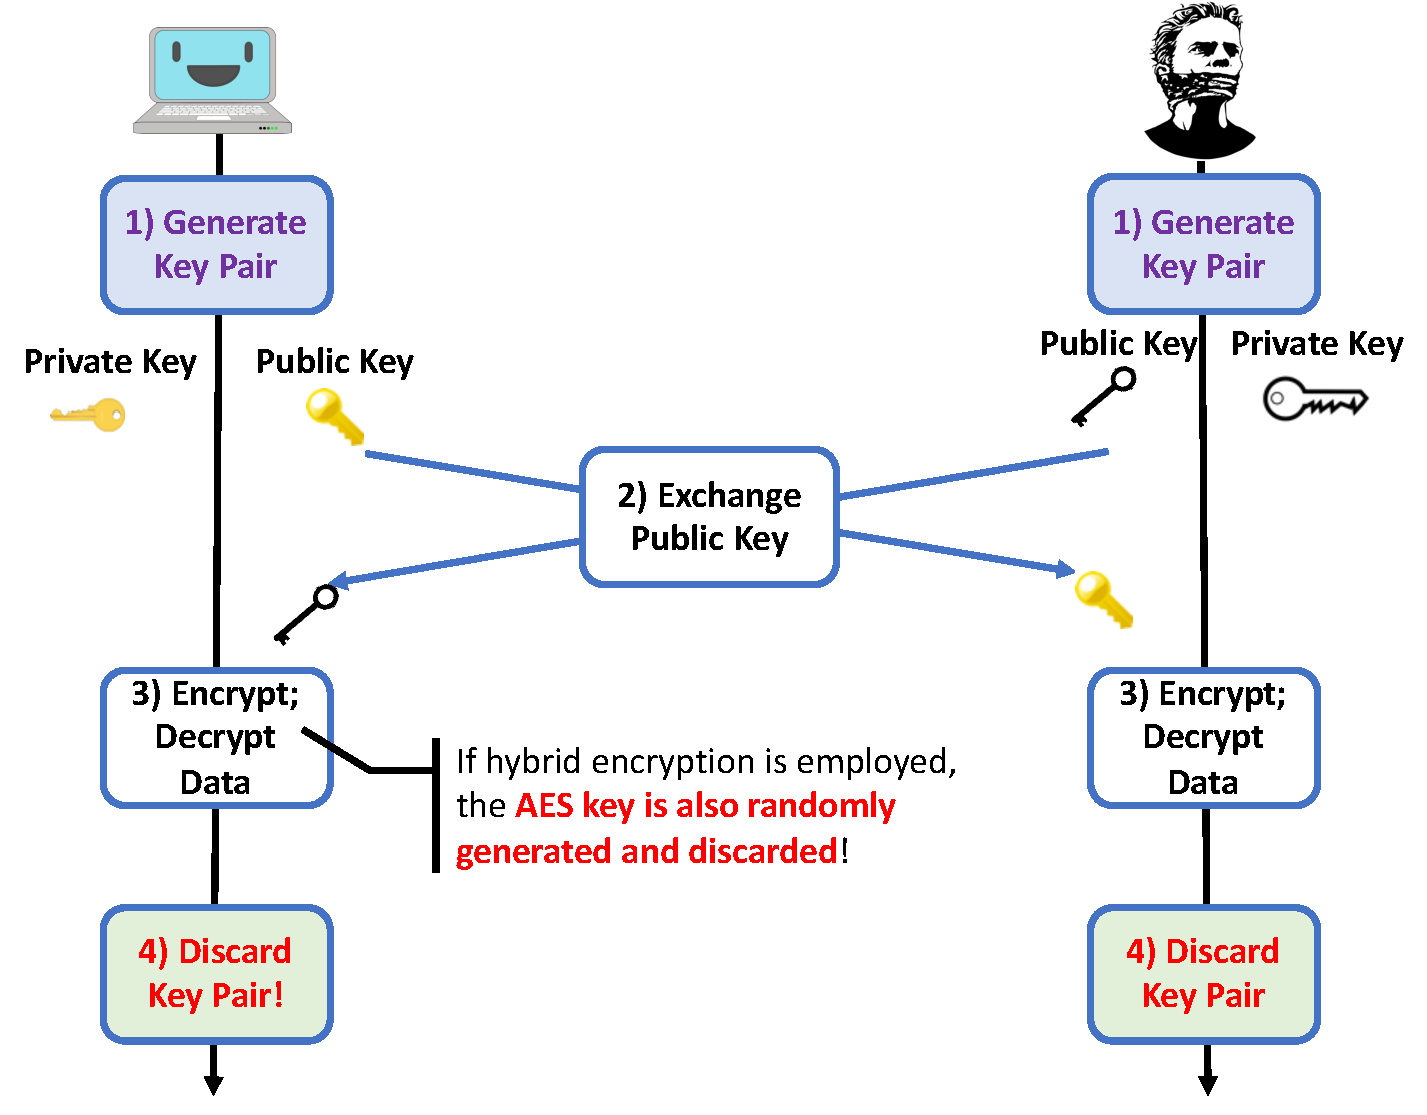
\includegraphics[width=0.7\linewidth]{Figs/ephemeral-scheme-flow01.pdf}\\
Ephemeral Schemeのイメージ
\end{center}
\vspace{-1ex}

まずはじめに、\alert{「送られてきたEphemeralな公開鍵は、本当に自分がやりとりしたい相手の公開鍵か?」の確認}が必須。\footnote[frame]{\scriptsize 意図しない相手の公開鍵で暗号化して機密データを漏らさぬように、ということ。}
\end{frame}

\begin{frame}

というわけで、「E2Eで安全にデータをやり取りする」ための基礎部分の最後のピースを今日は学ぶ。

\begin{block}{\small この講義で最終的に学びたいこと}
\begin{itemize}
\item 本人確認やデータの改ざん防止を担保する方法
\begin{itemize}
 \item データ毎に固有の指紋を生成する「\alert{ハッシュ}」
 \item 「共通鍵」を使った改ざん防止方法「\alert{MAC}」\footnote[frame]{\scriptsize HMAC (RFC2104 \url{https://tools.ietf.org/html/rfc2104})}
 \item 「公開鍵」を使った本人確認・改ざん防止方法「\alert{電子署名}」\footnote[frame]{\scriptsize RSASSA PKCS\#1-v1.5/PSS (PKCS\#1 RFC8017 \url{https://tools.ietf.org/html/rfc8017}), ECDSA (FIPS PUB186-4 \url{https://csrc.nist.gov/publications/detail/fips/186/4/final})}
\end{itemize}
\item そしてその具体的なJavaScriptでの実装方法・お作法
\end{itemize}
\end{block}

細かい話もするが、数式は使わない。

「イメージ」と「コードの流れ&その流れの必要性」をつかめるようにする。
\end{frame}

\begin{frame}
\frametitle{発表者紹介}
{\Large 栗原 淳 (Jun Kurihara)}
\begin{itemize}
 \item (株)ゼタント 主任研究員\\
(株) 国際電気通信基礎技術研究所(ATR) 連携研究員
 \item 博士(工学), \\
 専門: セキュリティ、応用数学、システムアーキテクチャとか
 \item  Webシステム(フロントエンド・バックエンド)を作ったり、論文他のアルゴリズムを実装したり、研究して論文書いたり、セキュリティ技術中心に手広くやってます。
 \item GitHub: \url{https://github.com/junkurihara}\\
LinkedIn: \url{https://www.linkedin.com/in/junkurihara}
\end{itemize}
\end{frame}

\begin{frame}
\frametitle{この講義の対象と事前準備}
対象:
\begin{itemize}
\item 暗号・セキュリティ技術に興味がある初学者
\item Webに暗号技術を導入したいWeb系のエンジニア
\end{itemize}

\vspace{2ex}

必須ではないが触って楽しむのには必要な事前準備:
\begin{itemize}
\item Bash, Gitが使えるようになっていること
\item Node.js, npm, yarnが使えるようになっていること
\item Google Chrome系ブラウザ and/or Firefoxが利用可能なこと
\end{itemize}
\end{frame}

\begin{frame}
今後の予定(暫定)
\begin{enumerate}
 \item \textcolor{gray}{導入\&JSの暗号化コードを触ってみる}
 \item \textcolor{gray}{AESを正しく・安全に暗号化するには?}
 \item \textcolor{gray}{公開鍵暗号はどうやって使う?その使い方のコツは?}
 \item \alert{ハッシュ・MAC・署名、それぞれの使い所と使い方は?} ← 今日はココ
 \item \textcolor{gray}{RFCにまつわるあれこれ(証明書・鍵フォーマット・etc...未定。)}
\end{enumerate}
「こういうのを知りたい」というリクエストがあれば是非。

\vspace{2ex}

\underline{セカンドシーズンも検討中。}\footnote[frame]{場所等変えてもっと来やすい場所へ。。。}
\end{frame}

%%%%%%%%%%%%%%%%%%%%%%%%%%%%%%%%%%%%%%%%%%%%%%%%%%%%%%%%%%%%%%%%%%%%%%%%%%%%%%%%%%%%%%%%%%%%%%%%%%%
\section{サンプルコードの準備}
\begin{frame}
\centering
{\Large サンプルコードの準備}
\end{frame}

\begin{frame}
\frametitle{準備}
\small
説明を聞きつつ手を動かすため、まず環境準備。
\alert{今回は、JavaScript (Node.js) を使って手元でデータのHash/MAC/署名をいじってみる。}
そしてその効果を実感する。

\begin{center}
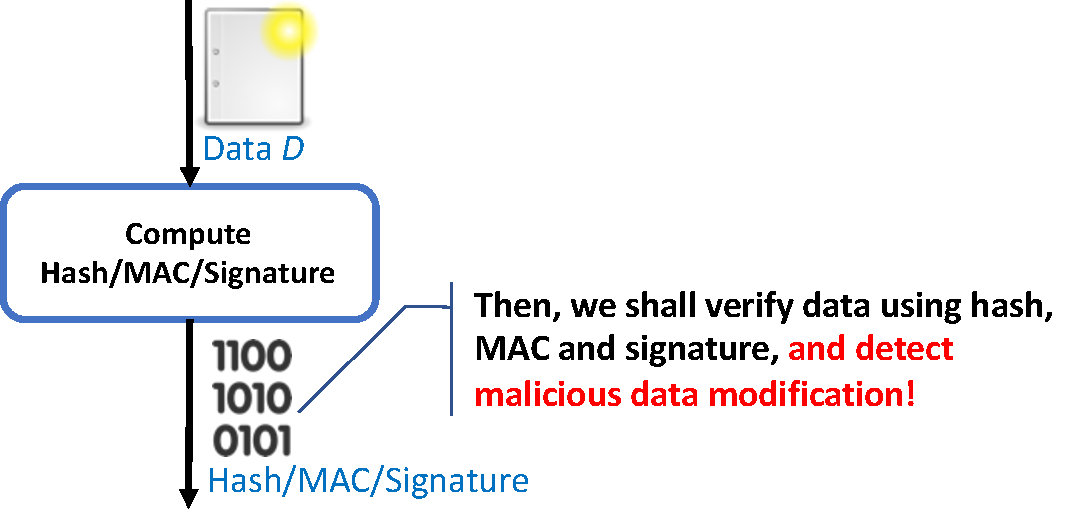
\includegraphics[width=0.7\linewidth]{Figs/md-flow.pdf}
\end{center}

\end{frame}

\begin{frame}

※\alert{サンプルコードはブラウザでも動く}。src/commands-browser.htmlを開くとこれからNode.JSで試すデモが開発者コンソールで実行される。適宜試したり比較すると良い。

\vspace{2ex}

※前回のコードの公開鍵に署名をつけたりしてEphemeral Schemeを作ってみると良い。
\end{frame}

\begin{frame}
\frametitle{環境}
以下の環境が前提:
\begin{itemize}
 \item Node.js ($>$ v10)がインストール済。yarnが使えること。 \footnote[frame]{インストールコマンド: \texttt{npm i -g yarn}}
 \item ブラウザとして、Google Chrome (系ブラウザ)、もしくはFirefoxがインストール済み
 \item Visual Studio Code や WebStorm などの統合開発環境がセットアップ済みだとなお良い。
\end{itemize}
\end{frame}

\begin{frame}
\frametitle{JavaScriptプロジェクトの準備}
\begin{enumerate}
\item プロジェクトのGitHubリポジトリ\footnote[frame]{\url{https://github.com/zettant/e2e-security-04}}をClone\\
\begin{exampleblock}{}
\footnotesize
\$ \texttt{git clone https://github.com/zettant/e2e-security-04}\\
\$ \texttt{cd e2e-security-04/sample}
\end{exampleblock}
\item 依存パッケージのインストール
\begin{exampleblock}{}
\$ \texttt{yarn install}
\end{exampleblock}
\item ライブラリのビルド
\begin{exampleblock}{}
\$ \texttt{yarn build}
\end{exampleblock}
\end{enumerate}
\end{frame}


%%%%%%%%%%%%%%%%%%%%%%%%%%%%%%%%%%%%%%%%%%%%%%%%%%%%%%%%%%%%%%%%%%%%%%%%%%%%%%%%%%%%%%%%%%%%%%%%%%%
\section{Hash}
\begin{frame}
\centering
{\Large データの指紋: Hash}
\end{frame}

\begin{frame}
\frametitle{HashおよびHash関数とは}
\begin{block}{\small HashおよびHash関数}
あるデータに対し、そのデータを「代表するビット列」を計算する不可逆の関数を「Hash関数」。導出したビット列を「Hash」\footnote[frame]{あるいはHash値、Message Digest}と呼ぶ。
\end{block}
\begin{center}
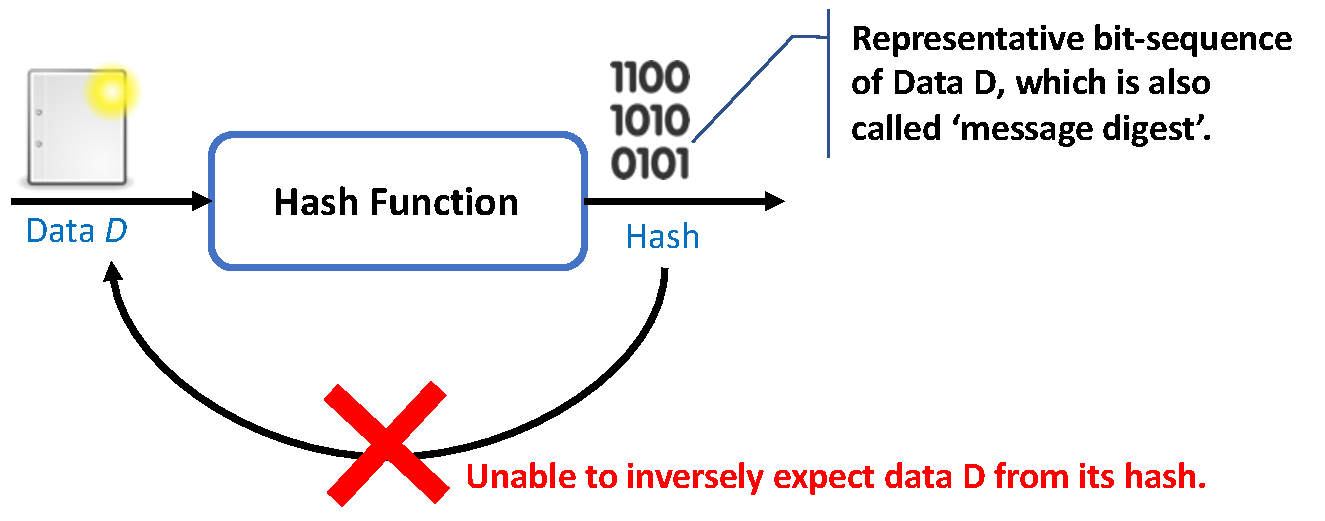
\includegraphics[width=0.8\linewidth]{Figs/hash-flow01.pdf}
\end{center}
\end{frame}

\begin{frame}
 1ビットでもデータが異なれば、全く違うHashが導出される。
\begin{center}
 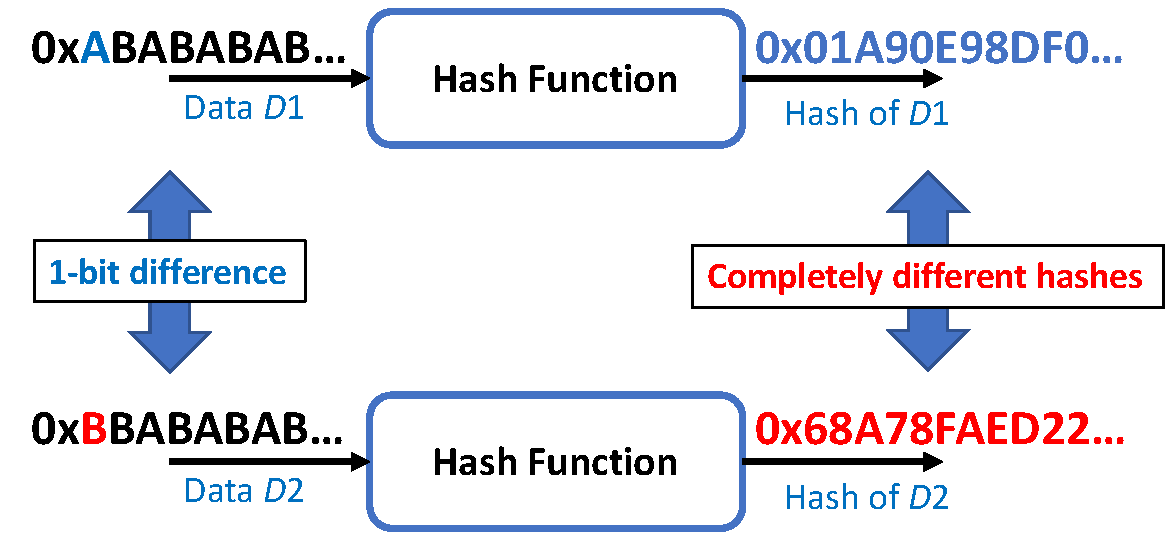
\includegraphics[width=0.8\linewidth]{Figs/hash-flow02.pdf}
\end{center}
\end{frame}

\begin{frame}
\small
\frametitle{HashおよびHash関数の役割}
同じくデータ固有のビット列を導出するChecksumと似ているが、その用途はより強力で多岐にわたる。

\begin{itemize}
 \item \textbf{Checksum}
\begin{itemize}
 \item 通信路上などでの\structure{データの(偶発的な)エラー検知}
\end{itemize}
$\Rightarrow$ \structure{データから一意に導ける値}・高速な処理が可能なことが必須
 \item \textbf{Hash}
\begin{itemize}
 \item \alert{データのエラー・改ざん検知}
 \item \alert{Hashをデータ実態の代替として署名を生成}
 \item 多数のデータの索引作成\footnote[frame]{Hash Table} 
 \item データの重複検出
\end{itemize}
$\Rightarrow$ \alert{別のデータ同士で同じHashを得ることが困難}なことが必須
\end{itemize}

\textbf{Checksum $\subseteq$ Hash} と言える。
\end{frame}

\begin{frame}
\frametitle{Hash関数の種類}
 MD5, SHA-1, SHA-2 (SHA-256, 384, 512), SHA-3というHash関数がよく知られている。
 \begin{center}
  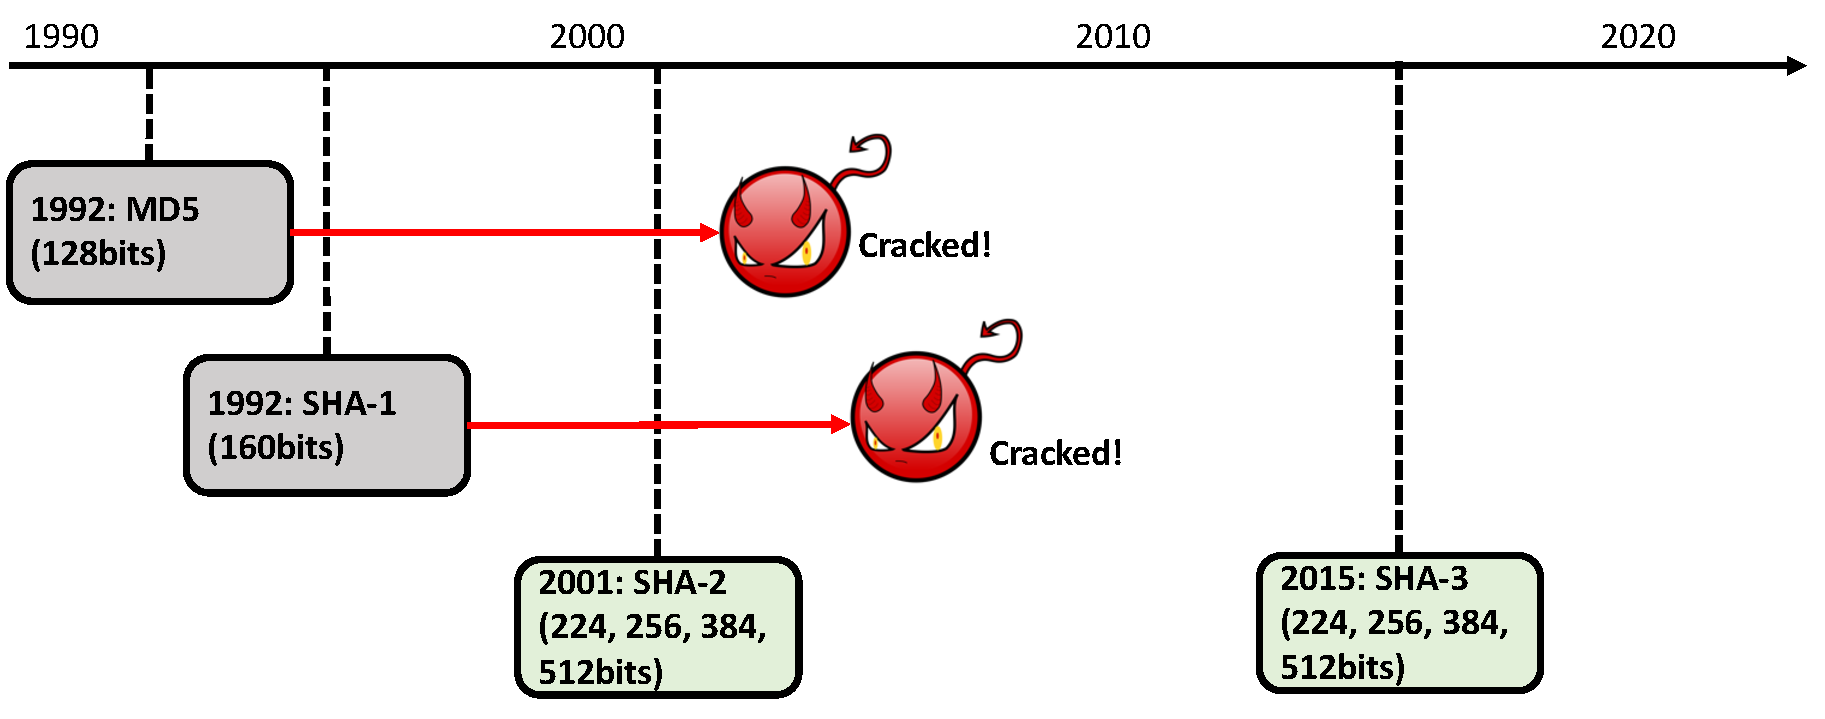
\includegraphics[width=\linewidth]{Figs/hash-history.pdf}
 \end{center}
 MD5、SHA-1は、「\alert{同じHash(指紋)を生成するデータが割と簡単に見つけられる}\footnote[frame]{「衝突」と呼ぶ。MD5の場合は、$2^{20}$程度の計算量でクラック可能。}」という致命的な欠陥が発見されている。
\end{frame}

\begin{frame}
\begin{block}{\small Hash関数の選択について}
\begin{itemize}
 \item 理由がなければSHA-2シリーズ以降のものを選択する。
\begin{itemize}
 \item bit長は長いほど、衝突するデータが見つけづらい(=強固)
 \item ただし、bit長が長いほど、計算が重くなる
\end{itemize}
 \item SHA-1/MD5は、基本的に互換性の担保のためだけに利用する。但し、Checksumとして使う分には概ね問題ない。\alert{何が何でも使うな、というわけではない。}
\end{itemize}
\end{block}

\begin{exampleblock}{\small IE/Edge こぼれ話}
\small
X.509の公開鍵証明書などはまだSHA-1が利用されている場合が多々ある。しかし、\alert{IE/Edgeでは互換性の担保を全て無視してSHA-1のネイティブサポートを全打ち切り}しているので、X.509公開鍵証明書などをJavaScriptからネイティブAPIを通して扱えない。
\end{exampleblock}
\end{frame}

\begin{frame}
\frametitle{JavaScriptでデータのHashを生成してみる。}
\end{frame}

\begin{frame}
Hash生成のコードはこんな感じ。
\end{frame}
%%%%%%%%%%%%%%%%%%%%%%%%%%%%%%%%%%%%%%%%%%%%%%%%%%%%%%%%%%%%%%%%%%%%%%%%%%%%%%%%%%%%%%%%%%%%%%%%%%%
\section{本人確認の技術}
\begin{frame}
\centering
{\Large 本人確認の技術}
\end{frame}

\begin{frame}
\frametitle{「正しい相手から正しく送信されてきたデータか」?}
いわゆる「データの真正性と送信元の確認方法」には、大まかに2つの方法がある。
\begin{itemize}
 \item Message Authentication Code (MAC)
 \item 署名 (電子署名)
\end{itemize}

\end{frame}

\begin{frame}
両者とも、送信するデータからMAC/署名という検証用データを生成、元データに付与する形で送信。
\begin{center}
 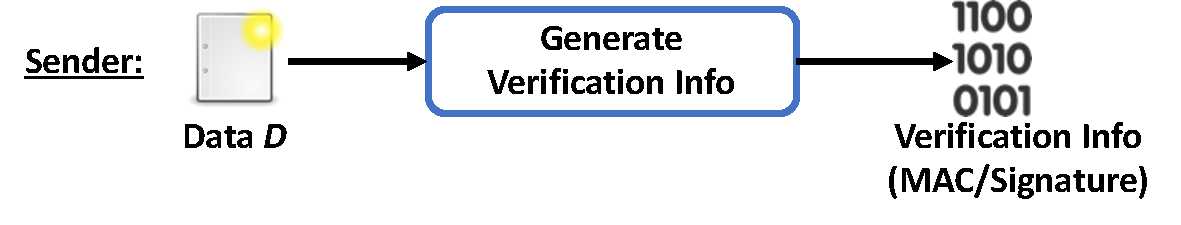
\includegraphics[width=0.75\linewidth]{Figs/mac-sig-flow01.pdf}
\end{center}
受信したデータと、MAC/署名とを突合して、「送信元は意図している相手か?」「データは改ざんされてないか?」を検証。
\begin{center}
 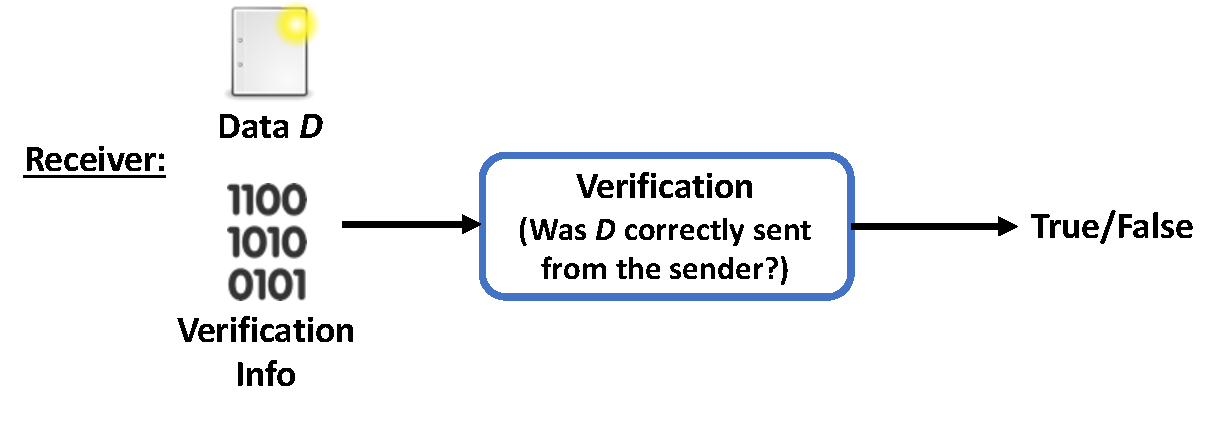
\includegraphics[width=0.75\linewidth]{Figs/mac-sig-flow02.pdf}
\end{center}
\end{frame}

\begin{frame}
MAC・署名の中身に突っ込む前に、それぞれのざっくりとした定義とpros/consを説明する。
\end{frame}

\begin{frame}
\frametitle{Message Authentication Code (MAC)}
\begin{block}{\small MACによるデータ真正性と送信者の確認}
\begin{itemize}
\item 送信側・受信側で共有する鍵を使って\alert{データ・鍵固有のバイナリ(MAC)}を生成する方法。
\item 受信側で、\alert{送信側と同一のMACが作れるかどうか}をチェック。
\end{itemize}
\end{block}
\begin{center}
 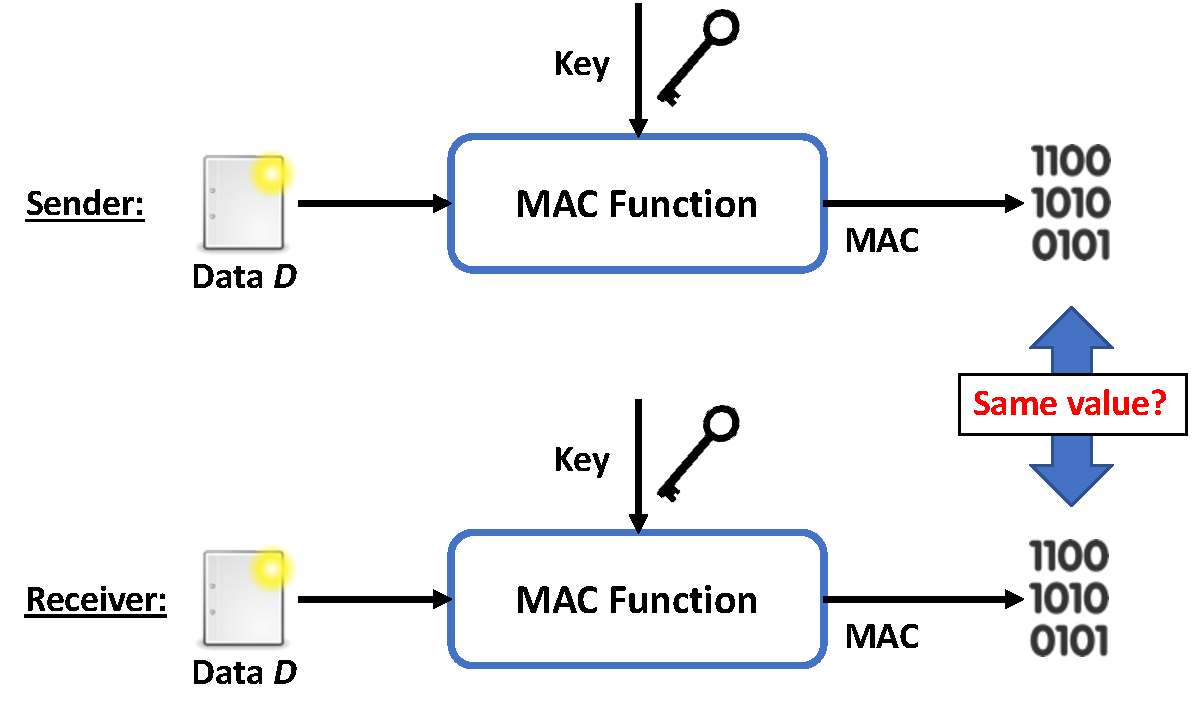
\includegraphics[width=0.7\linewidth]{Figs/mac-flow01.pdf}
\end{center}
\end{frame}
\begin{frame}
MACの特徴:
\begin{itemize}
 \item 同じ鍵でも、データが異なれば出力されるMACも異なる。
 \item 同じデータでも、鍵が異なれば出力されるMACも異なる。
\end{itemize}
\begin{center}
 $\Downarrow$
\end{center}
すなわち、受信側で同一のMACが作れることを確認できれば、\\
\begin{itemize}
 \item \alert{鍵を共有する相手}から
 \item \alert{途中の改ざんなしで送られたデータ}であること
\end{itemize}
が保証される。
\end{frame}

\begin{frame}
\frametitle{署名 (電子署名)}
公開鍵・秘密鍵ペアをベースとした技術\footnote[frame]{\scriptsize ここでいう公開鍵・秘密鍵ペアは、公開鍵暗号化に使うものと全く一緒の概念。}:
\begin{block}{署名によるデータ真正性と送信者の確認}
\begin{itemize}
 \item 送信側は公開鍵・秘密鍵ペアを保有。
 \item 送信側は、データと自分の秘密鍵から署名を生成。
 \item 受信側は、受信データ、署名と公開鍵の間の一貫性をチェック。
\end{itemize}
\end{block}
\begin{center}
 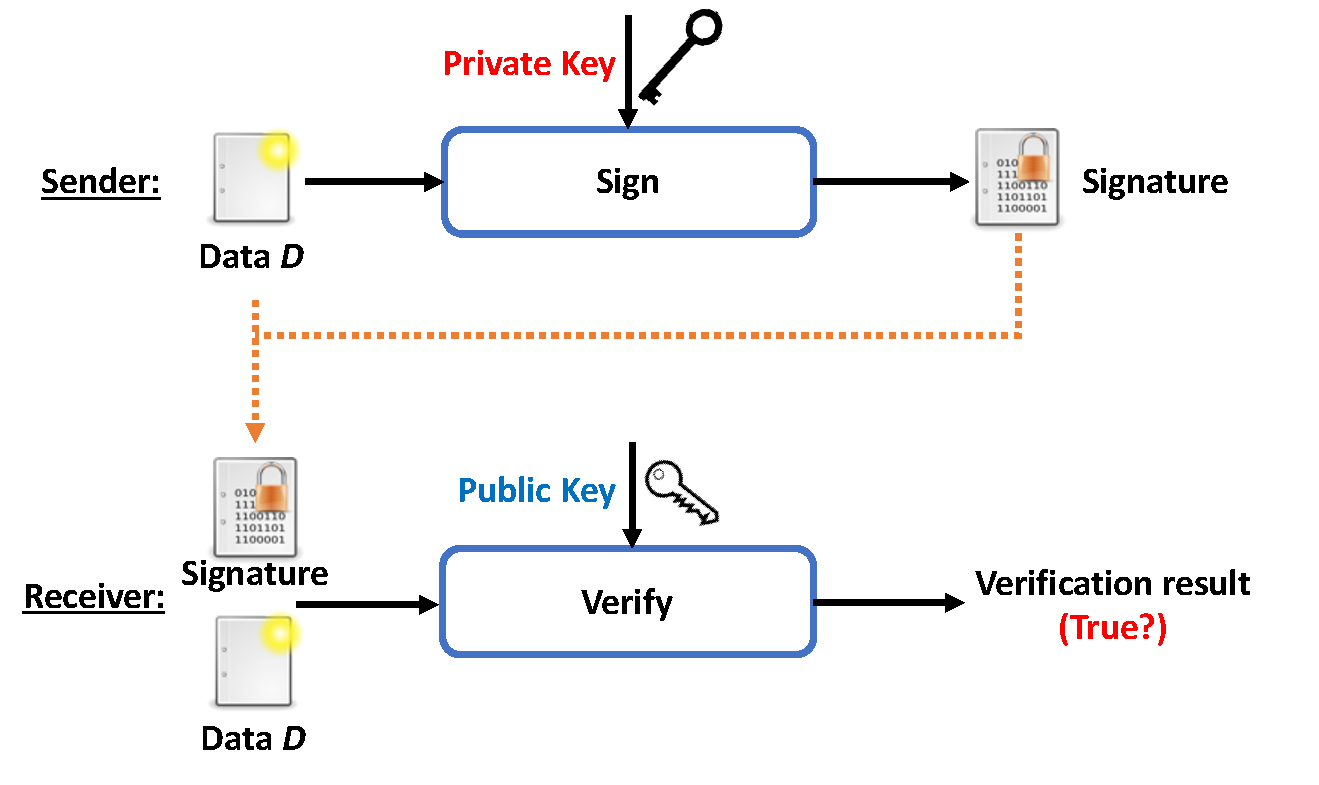
\includegraphics[width=0.63\linewidth]{Figs/sig-flow01.pdf}
\end{center}
\end{frame}

\begin{frame}
署名の特徴:
\begin{itemize}
 \item データが改ざんされていたら、検証が失敗(falseが出力)。
 \item 意図する相手の秘密鍵\footnote[frame]{\scriptsize 自分が入手している公開鍵の対となる秘密鍵}で署名が作られていなければ、検証が失敗。
 \item \alert{MACと違って、秘密の情報(=鍵)を事前共有しなくて良い}
\end{itemize}

\begin{center}
 $\Downarrow$
\end{center}
すなわち、署名技術は、\\
\begin{itemize}
 \item 意図する送信者から
 \item 途中の改ざんなしで送られたデータなことを
 \item \alert{事前の秘密情報の共有なし}で
\end{itemize}
保証する。\footnote[frame]{\scriptsize 検証用の公開鍵は、信頼できる手段で入手済み、あるいはプリインストールされていると仮定}
\end{frame}

\begin{frame}
\frametitle{MACと署名のpros/cons}
じゃあ署名だけでMACは不要では?…そういうわけにはいかない。
\begin{table}
\centering
\begin{tabular}{|p{0.07\linewidth}||p{0.39\linewidth}|p{0.43\linewidth}|}
\hline
 & \textbf{Pros} & \textbf{Cons}\\
\hline
\hline
\textbf{MAC}
& ・一般的に\alert{高速}\footnote[frame]{\scriptsize AES (CMAC) とかHash (HMAC) とかを構成要素としているため。} & ・鍵の\structure{事前共有が必要} \\
& ・生成するMACサイズは{小さい}\footnote[frame]{\scriptsize 通常128--512bits程度。} & \\
\hline
\textbf{署名}
& ・鍵の\alert{事前共有が不要} & ・一般的に\structure{非常に遅い・重い}\\
& & ・生成する署名サイズは一般的に\structure{大きい}\footnote[frame]{\scriptsize ECDSAは小さく、256--512bits程度。RSA系は非常に大きく通常2048bits以上。} \\
\hline
\end{tabular}
\end{table}

$\Rightarrow$ AES/公開鍵暗号の関係と全く一緒で、使い所を考えて組み合わせて使う、もしくは場合に応じて使い分ける。

\end{frame}


%%%%%%%%%%%%%%%%%%%%%%%%%%%%%%%%%%%%%%%%%%%%%%%%%%%%%%%%%%%%%%%%%%%%%%%%%%%%%%%%%%%%%%%%%%%%%%%%%%%
\section{MAC}
\begin{frame}
\centering

{\Large 共通鍵を使った改ざん検知・本人確認: MAC}

\end{frame}

\begin{frame}
\frametitle{Message Authentication Code (MAC) 事始め}
\begin{block}{\small MACを使った改ざん検知\&本人確認手続き}
\small
送信側、受信側で秘密の鍵(バイナリ列)を共有。
\begin{enumerate}
\item 送信側はデータと一緒に、データと鍵から生成したMACを送信。
\item 受信側は、鍵と受信したデータから、受け取ったMACと同じものが作れるかどうかをチェック。
\end{enumerate}
\end{block}

\begin{center}
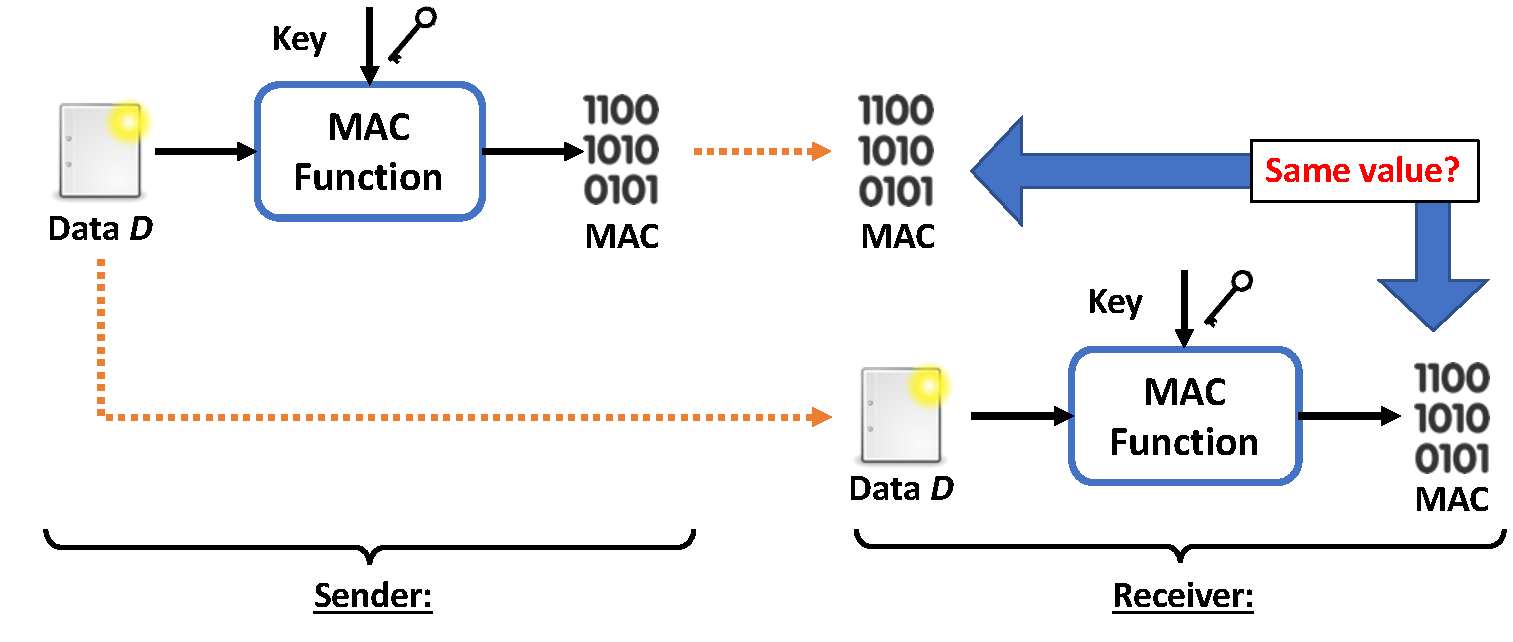
\includegraphics[width=0.9\linewidth]{Figs/mac-flow02.pdf}
\end{center}
\end{frame}

\begin{frame}
MACを作る標準手法のバリエーション。 
\begin{itemize} 
 \item \alert{HMAC; Hash-based Message Authentication Code}
 \item CMAC; Cipher-based Message Authentication Code
 \item GMAC; Galois Message Authentication Code
 \item etc.
\end{itemize}
今回は、JSで一番使いやすいと思われるHMACを取り上げる。
\end{frame}


\begin{frame}
\frametitle{HMAC; Hash-based MAC}
\begin{block}{\small HMAC (RFC2104)\footnote[frame]{\scriptsize \url{https://tools.ietf.org/html/rfc2104}}}
\begin{itemize}
 \item 鍵付きHash\footnote[frame]{\scriptsize Keyed Hash}と呼ばれる、Hash関数ベースのMAC生成方法。
 \item HDKF (RFC5869)などの標準技術や、AWS Signature v4\footnote[frame]{\scriptsize AWS S3にクライアントからREST API経由でアップロードする時に一時的に生成するMAC}等、各所で利用されている。
\end{itemize}
\end{block}
\underline{「鍵」と「データ」をまとめてHash関数に入れる}、と考えると、
\begin{itemize}
 \item 鍵・データ両者が正しくないと、正しいHashも生成不能(=MAC検証失敗)。
 \item MACから鍵・データの情報を逆算することはできない。
\end{itemize}
という特徴をイメージしやすい。
\end{frame}

\begin{frame}
\frametitle{JavaScriptでHMACを実行してみる}
\end{frame}

\begin{frame}
コードの中身はこんな感じ。
\end{frame}

\begin{frame}
\frametitle{その他のMAC (JSじゃビミョー…)}
\begin{block}{\small CMAC; Cipher-based MAC (NIST SP800-38B\footnote[frame]{\scriptsize https://nvlpubs.nist.gov/nistpubs/SpecialPublications/NIST.SP.800-38b.pdf})}
\alert{共通鍵暗号(e.g., AES)のCBCモードをHash関数がわりに使用}してMACを計算する。
「前のブロックの暗号文を使って次のブロックを暗号化する」という特徴を応用。
\end{block}

\begin{block}{\small GMAC; Galois MAC (NIST SP800-38D\footnote[frame]{\scriptsize https://nvlpubs.nist.gov/nistpubs/Legacy/SP/nistspecialpublication800-38d.pdf})}
共通鍵暗号(e.g., AES)の Galois Counter Mode (GCM) で暗号化と同時に生成されるMAC。
\alert{高速に計算できる代数演算\footnote[frame]{\scriptsize $\mathbb{F}[x]/(x^{128}\!+\!x^7\!+\!x^2\!+\!x\!+\!1) = \mathbb{F}_{2^{128}}$上の乗算}をHash関数がわりに使用}してMACを計算する。
GMAC単独で利用可。
\end{block}

\end{frame}

\begin{frame}

と、「標準技術」で「広く利用されている」MACアルゴリズムはあるが、\structure{JSのネイティブAPI\footnote[frame]{\scriptsize WebCrypto API, Node.js Crypto}でサポートされているMACは、現状HMACのみ…}

\vspace{2ex}

CMAC, GMACが使いたかったら自力実装 or npmjs.comで見つけて利用する。
\end{frame}

%%%%%%%%%%%%%%%%%%%%%%%%%%%%%%%%%%%%%%%%%%%%%%%%%%%%%%%%%%%%%%%%%%%%%%%%%%%%%%%%%%%%%%%%%%%%%%%%%%%
\section{署名}
\begin{frame}
\centering
{\Large 公開鍵を使った改ざん検知・本人確認: 署名}

\end{frame}

\begin{frame}
\frametitle{署名 事始め}

\begin{block}{\small 署名 (電子署名) を使った改ざん検知\&本人確認手続き}
受信側は、送信側の公開鍵を予めプリインストール。
\begin{itemize}
 \item 送信側の処理:
\begin{enumerate}
 \item データ$D$をHash関数で短縮\footnote[frame]{\scriptsize データ$D$そのものに直接署名を施すのは計算量的・データ量的に大変(e.g, 元データと同じかそれ以上の大きさの署名を作る羽目になる)なので、\alert{データの指紋(i.e., hash)に対して署名を施す}。}。
$h = \mathit{Hash}(D)$
 \item hash $h$に対して秘密鍵$\mathit{SK}$で署名を生成、データと合わせて受信側へ送付。$s = \mathit{Sign}(h, \mathit{SK})$
\end{enumerate}
 \item 受信側の処理:
\begin{enumerate}
 \item データ$D$をHash関数で短縮。
$h = \mathit{Hash}(D)$
 \item hash $h$と署名 $s$の一貫性を、公開鍵$\mathit{PK}$で検証。$\mathit{Verify}(h, s, \mathit{PK}) \in \{\mathsf{True}, \mathsf{False}\}$
\end{enumerate}
\end{itemize}
\end{block}
\end{frame}

\begin{frame}
ざっくりフロー図。
\begin{center}
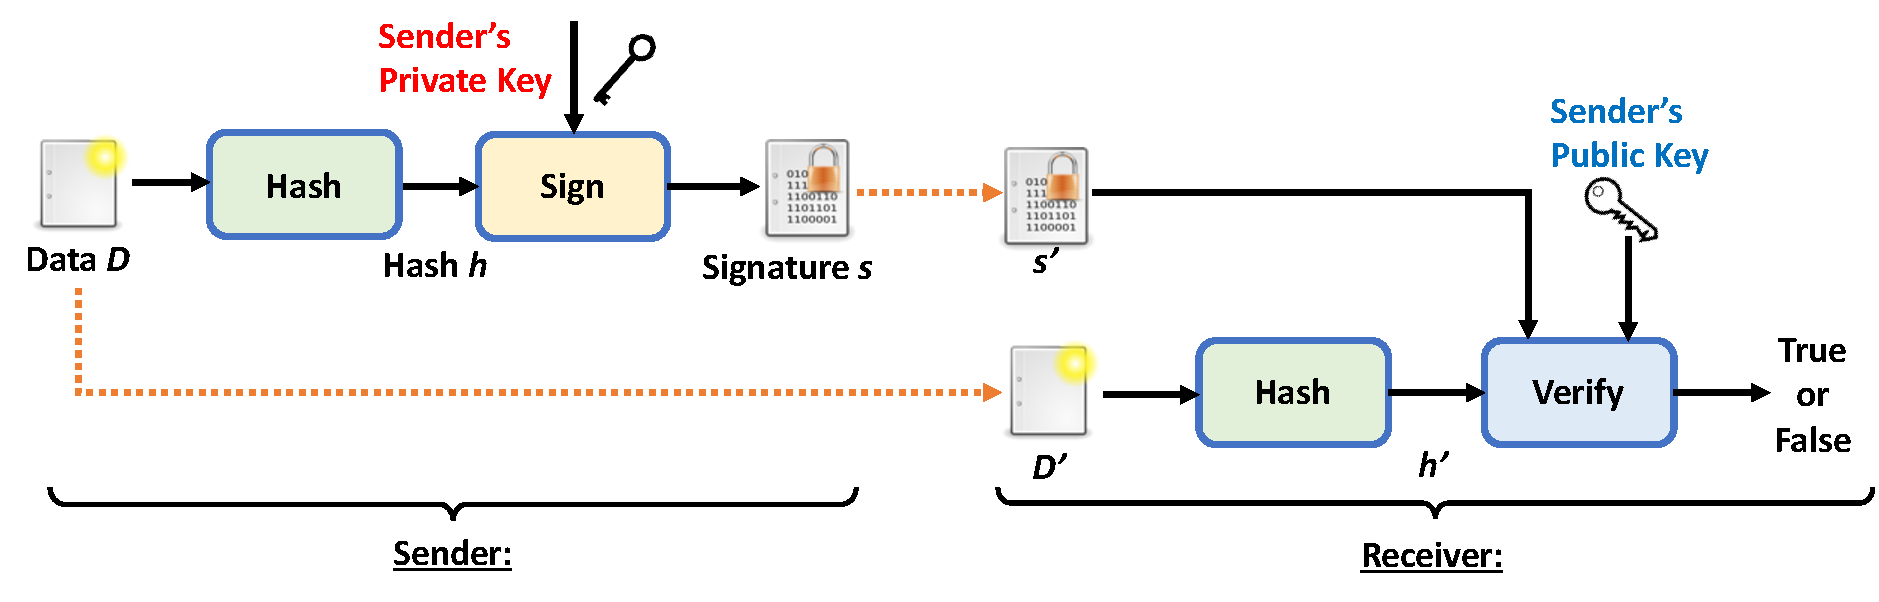
\includegraphics[width=0.9\linewidth]{Figs/sig-flow02.pdf}
\end{center}
このフローは、以下のように考えるとイメージがつきやすい\footnote[frame]{\scriptsize 但し、常に正しい表現ではないので注意。}
\begin{enumerate}
 \item 送信側は、hash $h$を\alert{秘密鍵で暗号化}して$s$を生成。
 \item 受信側は、$s$を\structure{公開鍵で復号}して$h'$を入手。命題「$h' = \mathit{Hash}(D')$」が成立するか検証。
\end{enumerate}
\end{frame}

\begin{frame}
署名生成方式の標準方式のバリエーション。
\begin{itemize}
\item RSA暗号をベースとした手法:
\begin{itemize}
 \item RSASSA PSS
 \item RSASSA PKCS\#1-v1.5
\end{itemize}
\item 楕円曲線暗号をベースとした手法:
\begin{itemize}
 \item ECDSA
\end{itemize}
\item etc.\footnote[frame]{\scriptsize Digital Signature Algorithm; DSA (FIPS PUB 186-4 \url{https://nvlpubs.nist.gov/nistpubs/FIPS/NIST.FIPS.186-4.pdf})など}
\end{itemize}
JSで使いやすいRSASSA PSS \& PKSC\#1-v1.5とECDSAについて取り上げる。
\end{frame}


\begin{frame}
\frametitle{RSASSA; RSA Signature Scheme with Appendix}
\begin{block}{\scriptsize RSASSA PKCS\#1-v1.5と、RSASSA PSSの違い}
暗号化と同様に、$h=\mathit{Hash}(D)$に対して署名を作る際、\underline{鍵長に合わせたパディングが必要}。そのパディングの方法が違う。
\end{block}

\alert{絵}

\end{frame}

\begin{frame}
\alert{PKCS\#1 - v1.5の脆弱性について}

  % Note: As noted in PKCS #1 v1.5, the EMSA-PKCS1-v1_5 encoding method
  %  has the property that the encoded message, converted to an integer
  %  message representative, is guaranteed to be large and at least
  %  somewhat "random".  This prevents attacks of the kind proposed by
  %  Desmedt and Odlyzko [CHOSEN] where multiplicative relationships
  %  between message representatives are developed by factoring the
  %  message representatives into a set of small values (e.g., a set of
  %  small primes).  Coron, Naccache, and Stern [PADDING] showed that a
  %  stronger form of this type of attack could be quite effective against
  %  some instances of the ISO/IEC 9796-2 signature scheme.  They also
  %  analyzed the complexity of this type of attack against the
  %  EMSA-PKCS1-v1_5 encoding method and concluded that an attack would be
  %  impractical, requiring more operations than a collision search on the
  %  underlying hash function (i.e., more than 2^80 operations).
  %  Coppersmith, Halevi, and Jutla [FORGERY] subsequently extended Coron
  %  et al.'s attack to break the ISO/IEC 9796-1 signature scheme with
  %  message recovery.  The various attacks illustrate the importance of
  %  carefully constructing the input to the RSA signature primitive,
  %  particularly in a signature scheme with message recovery.
  %  Accordingly, the EMSA-PKCS-v1_5 encoding method explicitly includes a
  %  hash operation and is not intended for signature schemes with message
  %  recovery.  Moreover, while no attack is known against the
  %  EMSA-PKCS-v1_5 encoding method, a gradual transition to EMSA-PSS is
  %  recommended as a precaution against future developments.

可能ならPSSを利用することが、RFCで推奨されている。\footnote[frame]{\scriptisize https://tools.ietf.org/html/rfc8017#section-8.2}
\end{frame}

\begin{frame}
\frametitle{JavaScriptでRSASSA-PSSを実行してみる}
\end{frame}

\begin{frame}
\frametitle{ECDSA}
\end{frame}

\begin{frame}
\frametitle{JavaScriptでECDSAを実行してみる}
\end{frame}



\begin{frame}
 {\Large 運用Tips}
\end{frame}

\begin{frame}
\frametitle{署名検証のブートストラップの問題}

\alert{署名の検証用の公開鍵が正しいことはどうやって保証するの?}

\vspace{2ex}

$\Rightarrow$ Appに固定インストールか、Verisignあたりに署名してもらう必要…

\vspace{2ex}

$\Rightarrow$ PKIに頼って検証用の公開鍵の信頼性を担保するしか、現状は方法がない。

\end{frame}

\begin{frame}
\frametitle{署名・MACの使い分け}
処理の重さで使い分けると幸せになれる。

\begin{itemize}
 \item \alert{署名は手続きのイニシエーション}に使う
 \item \structure{MACは、なんども繰り返すような本人確認}に使う
\end{itemize}

\vspace{2ex}

例えば。。。

\begin{enumerate}
\item 署名を付与して、ECDH-ephemeralの公開鍵を交換。
\item ECDH-ephemeral + AESでMACの鍵を共有。
\item 以降の大規模データのやり取りはMACで本人確認を実施。
\end{enumerate}

など。
\end{frame}


%%%%%%%%%%%%%%%%%%%%%%%%%%%%%%%%%%%%%%%%%%%%%%%%%%%%%%%%%%%%%%%%%%%%%%%%%%%%%%%%%%%%%%%%%%%%%%%%%%%
\section{まとめ}
\begin{frame}
 \centering
 {\Large まとめ}
\end{frame}

\begin{frame}
\frametitle{まとめ}
お疲れ様でした。

\begin{itemize}
\item 
\end{itemize}
\end{frame}


\begin{frame}
\frametitle{次回は}
% \begin{itemize}
%  \item 内容: 
% \begin{itemize}
%  \item 暗号化に加えて、MAC・署名を使ってみよう(数学的なことはやらない)
%  \item まずはハッシュ: SHA2, SHA3
%  \item 共通鍵ベース: HMAC/CMAC
%  \item 公開鍵ベース: RSA Signature/ECDSA
% \end{itemize}
%  \item 日時: 2019年10月31(?)日(木曜日) 19:00- (2週間後)
%  \item 場所: ブロックチェーンハブ (ここ)
%  \item 発表者: (また) 栗原
% \end{itemize}
\end{frame}


\begin{frame}
\frametitle{宣伝: iTransfy by Zettant}
\begin{center}
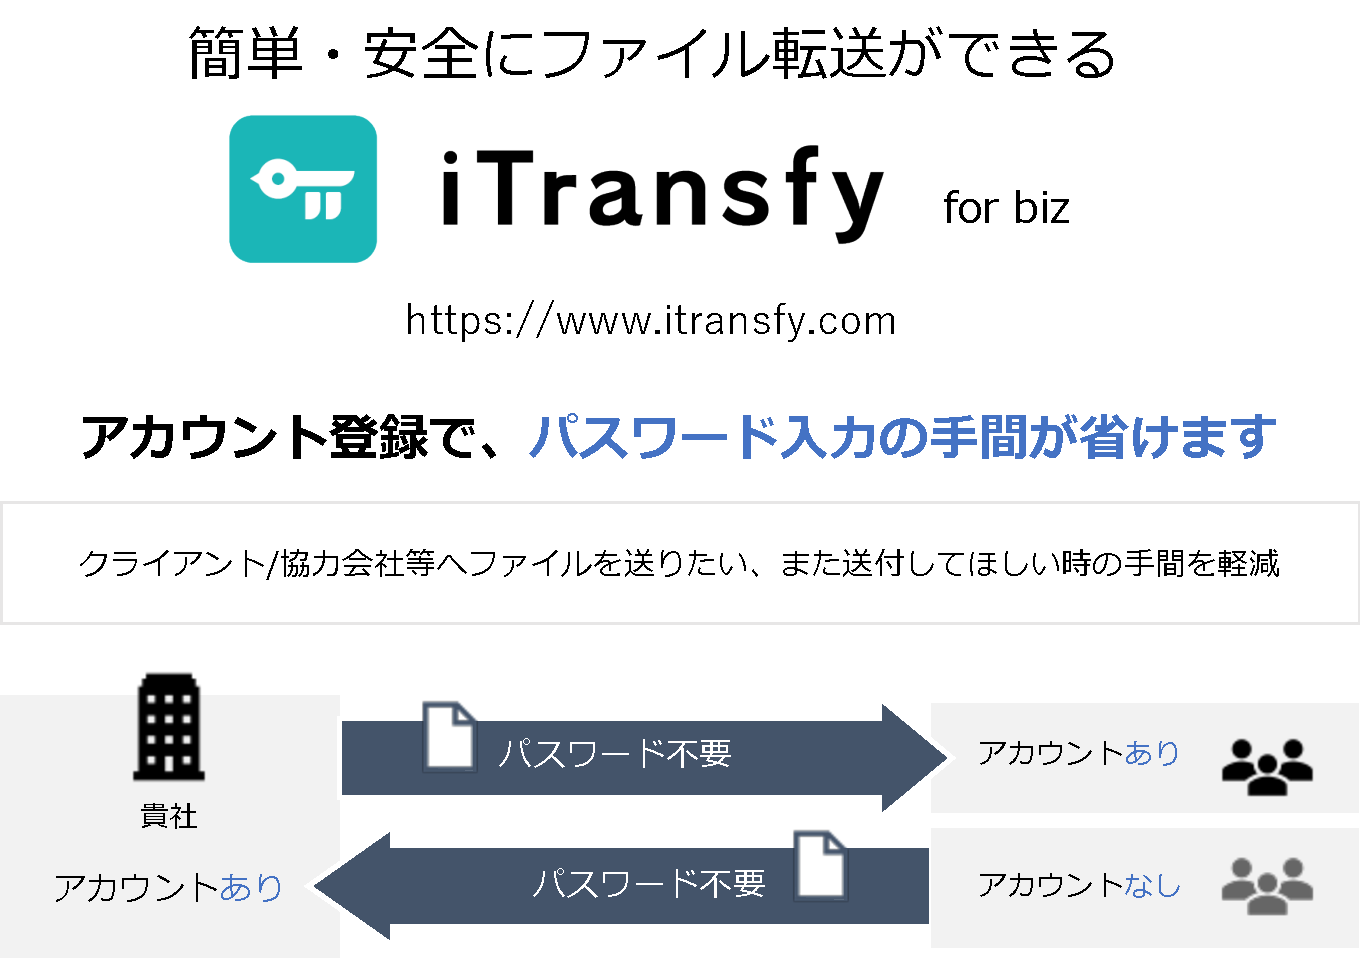
\includegraphics[width=0.9\linewidth]{FigsZettant/itransfy.pdf} 
\end{center}
\end{frame}

\begin{frame}
\frametitle{宣伝: 株式会社ゼタント}
\begin{tabular}{cc}
\begin{minipage}[b]{0.3\linewidth}

\includegraphics[width=\linewidth]{FigsZettant/logo.pdf}
\vspace{1ex}
\end{minipage}
 & 
\begin{minipage}[b]{0.7\linewidth}
\footnotesize
ゼタントはのミッションは、\\

「自分の身は自分で守ることができる世の中にする」\\

ことです。\\
共感してくれる仲間を募集しています!\\

問合せ先: \url{recruit@zettant.com}\\
会社URL: \url{https://www.zettant.com}
\end{minipage}
\end{tabular}
\end{frame}








% %%%%%%%%%%%%%%%%%%%%%%%%%%%%%%%%%%%%%%%%%%%%%%%%%%%%%%%%%%%%%%%%%%%%%%%%%%%%%%%%%%%%%%%%%%%%%%%%%%%
% \backupbegin

% \begin{frame}
%  以下バックアップ
% \end{frame}
% \begin{frame}
% 直接Concat KDFを暗号化の鍵にするか、
% あるいはConcat KDFの結果をAESKWの鍵としてContent Encryption Keyを暗号化するのに使う。

% \end{frame}

% \begin{frame}
% \frametitle{ECDH Ephemeral (ECDHE)}
% \begin{center}
% 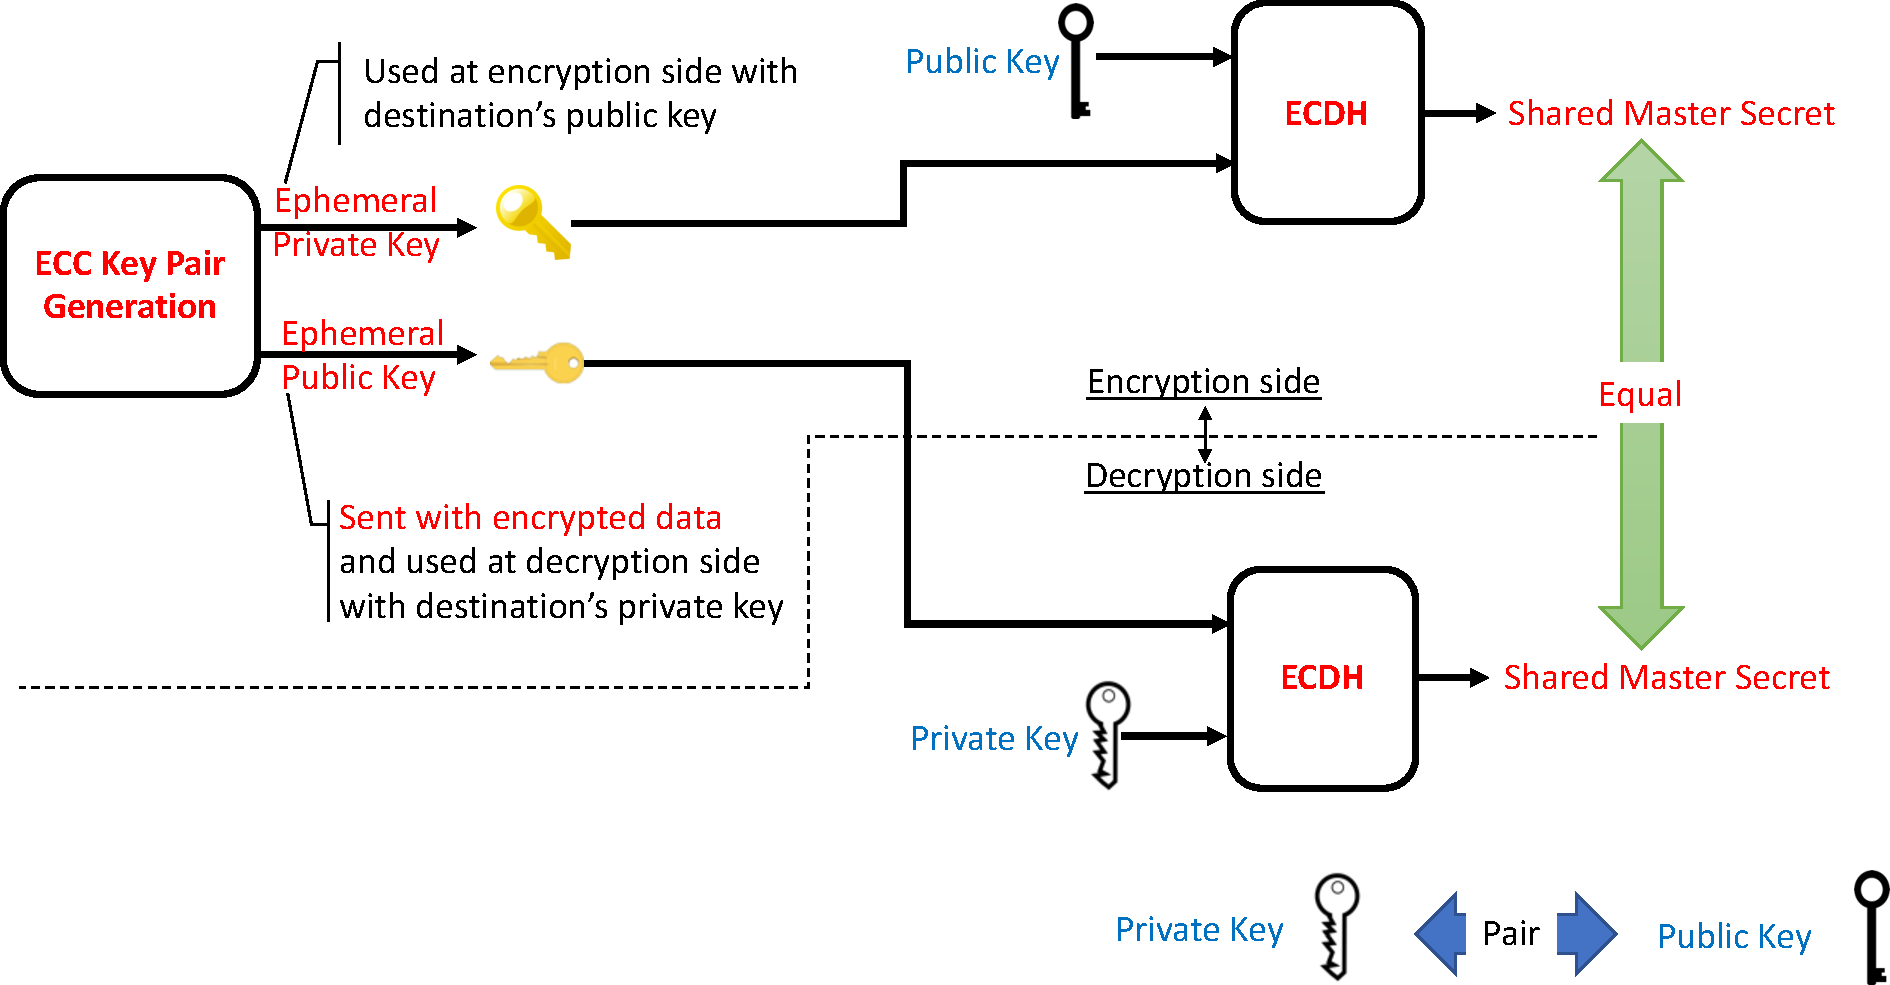
\includegraphics[width=\linewidth]{Figs/ecdh01.pdf}
% \end{center}
% \end{frame}

% \begin{frame}
% \begin{center}
% 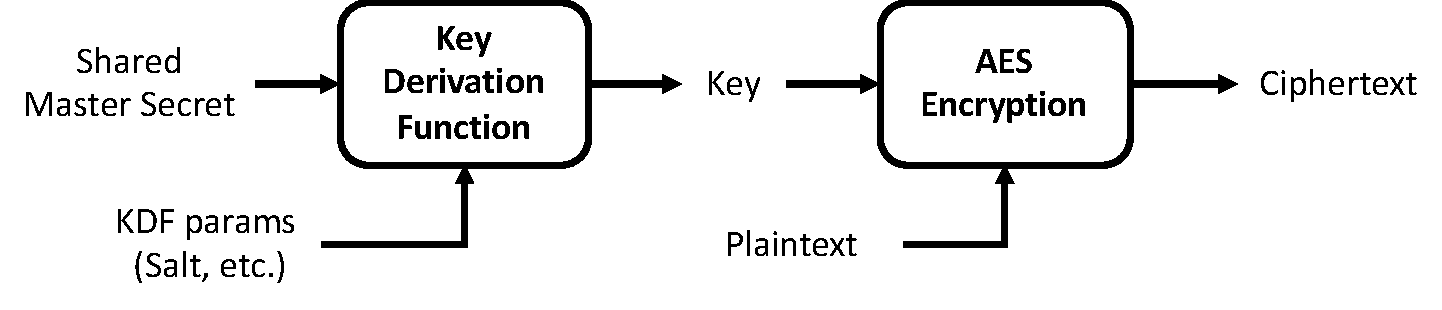
\includegraphics[width=\linewidth]{Figs/ecdh02.pdf}
% \end{center}
% \end{frame}


% \begin{frame}
% \begin{center}
% 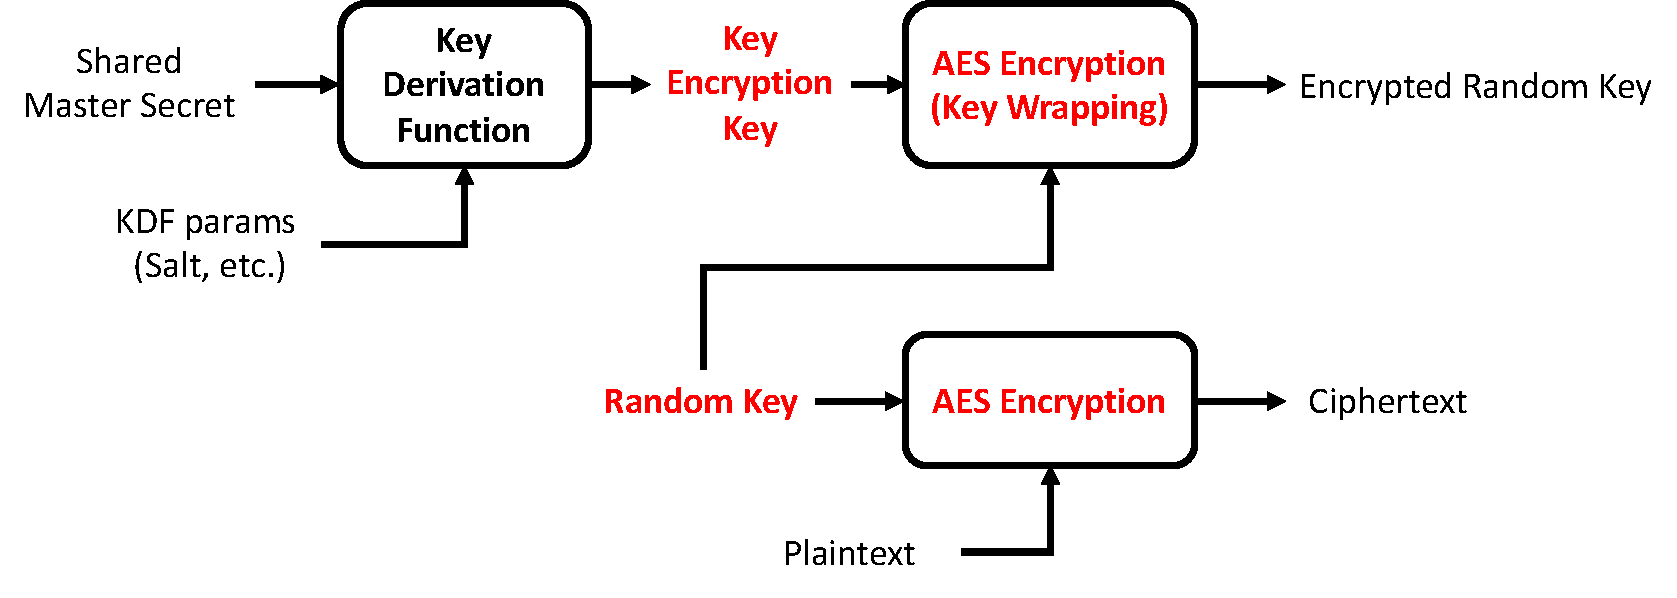
\includegraphics[width=\linewidth]{Figs/aeskw.pdf}
% \end{center}
% \end{frame}




% \section{Backup}

% \begin{frame}
 
% \end{frame}

% \begin{frame}
% \frametitle{Appendix}
% This page is not counted.
% \end{frame}
% \backupend
\end{document}
%%%%%%%%%%%%%%%%%%%%%%%%%%%%%%%%%%%%%%%%%%%%%%%%%%%%%%%%%%%%%%%%%%%%%%%%%%%%%%%%%%%%%%%%%%%%%%%%%%%
%%%%%%%%%%%%%%%%%%%%%%%%%%%%%%%%%%%%%%%%%%%%%%%%%%%%%%%%%%%%%%%%%%%%%%%%%%%%%%%%%%%%%%%%%%%%%%%%%%%
%%%%%%%%%%%%%%%%%%%%%%%%%%%%%%%%%%%%%%%%%%%%%%%%%%%%%%%%%%%%%%%%%%%%%%%%%%%%%%%%%%%%%%%%%%%%%%%%%%%
%%%%%%%%%%%%%%%%%%%%%%%%%%%%%%%%%%%%%%%%%%%%%%%%%%%%%%%%%%%%%%%%%%%%%%%%%%%%%%%%%%%%%%%%%%%%%%%%%%%
%%%%%%%%%%%%%%%%%%%%%%%%%%%%%%%%%%%%%%%%%%%%%%%%%%%%%%%%%%%%%%%%%%%%%%%%%%%%%%%%%%%%%%%%%%%%%%%%%%%
%%%%%%%%%%%%%%%%%%%%%%%%%%%%%%%%%%%%%%%%%%%%%%%%%%%%%%%%%%%%%%%%%%%%%%%%%%%%%%%%%%%%%%%%%%%%%%%%%%%
